\documentclass[border=3mm,tikz,preview]{standalone}
\usetikzlibrary{intersections}
\usepackage{amsmath}
\usetikzlibrary{shapes.misc}
\usetikzlibrary{arrows}

\tikzset{cross/.style={cross out, draw=black, minimum size=2*(#1-\pgflinewidth), inner sep=0pt, outer sep=0pt},
	%default radius will be 1pt. 
	cross/.default={2pt}}

\begin{document}
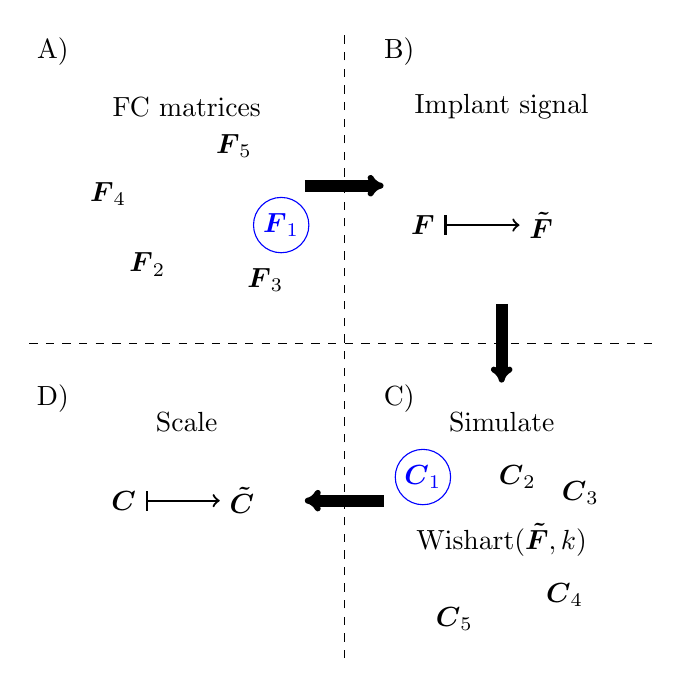
\begin{tikzpicture}
%	\draw[thin,gray!40] (-4,-4) grid (4,4);
	\draw[dashed] (-4,0)--(4,0);
	\draw[dashed] (0,-4)--(0,4);
%	\filldraw[black] (-1,1) circle (2pt) node{$\boldsymbol{F}_1$};
%	\draw[black] (-0.8,2) node{$\boldsymbol{F}_1$};

%% Image labels
	\draw (-3.7, 3.7) node{A)};
	\draw (0.7, 3.7) node{B)};
	\draw (-3.7, -0.7) node{D)};
	\draw (0.7, -0.7) node{C)};

%% FC nodes
	\draw (-2, 3) node{FC matrices};
	\draw[black] (-2.5,1) node{$\boldsymbol{F}_2$};
	\draw[black] (-1,0.8) node{$\boldsymbol{F}_3$};
	\draw[black] (-3,1.9) node{$\boldsymbol{F}_4$};
	\draw[black] (-1.4,2.5) node{$\boldsymbol{F}_5$};
	
%% Implant signal
	\draw (2, 3) node{Implant signal};
	
%% Simulates
	\draw (2, -1) node(simulate-title){Simulate};
	\draw[black] (2.2,-1.7) node{$\boldsymbol{C}_2$};
	\draw[black] (3,-1.9) node{$\boldsymbol{C}_3$};
	\draw[black] (2.8,-3.2) node{$\boldsymbol{C}_4$};
	\draw[black] (1.4, -3.5) node{$\boldsymbol{C}_5$};
	
%% Scale
	\draw (-2, -1) node{Scale};
	
%% Named nodes
	\draw[blue]   (-0.8,1.5) circle (10pt) node (baseline){$\boldsymbol{F}_1$};
	\draw[black]  (1,1.5)  node (implant){$\boldsymbol{F}$} ;
	\draw[black]  (2.5, 1.5)  node (implantsignal){$\boldsymbol{\tilde{F}}$} ;
	\draw[black] (2, -2.5) node (wishart){$\mathrm{Wishart}(\boldsymbol{\tilde{F}}, k)$};
	\draw[blue] (1,-1.7) circle (10pt) node (simulate){$\boldsymbol{C}_1$};
	\draw[black]  (-2.8,-2)  node (c){$\boldsymbol{C}$} ;
	\draw[black]  (-1.3, -2)  node (scaledc){$\boldsymbol{\tilde{C}}$} ;
%	\draw[black, |->]  (1.5,2) -- (2.5, 2)  node (implantsignal){$\boldsymbol{\tilde{F}}$} ;
	
	
	% Lines
%	\draw[|->, thick,] (baseline.east) .. controls +(up:-2mm) and +(up:7mm) .. (implant.north);
	\draw[-implies, thick,line width=0.15cm,]  (-0.5, 2)--(0.5, 2);
	\draw[-implies, thick,line width=0.15cm]  (2, 0.5)--(2, -0.5);
	\draw[-implies, thick,line width=0.15cm] (0.5, -2)--(-0.5, -2);
%	\draw[->, thick,] (simulate.west) .. controls +(down:-2mm) and +(up:7mm) .. (c.north);
%	\draw[->, thick,] (implantsignal.south) .. controls +(down:5mm) and +(right:7mm) .. (simulate-title.east);
	\draw[|->, thick] (implant.east) .. controls +(right:0mm) and +(left:0mm) .. (implantsignal.west);
	\draw[|->, thick] (c.east) .. controls +(right:0mm) and +(left:0mm) .. (scaledc.west);
%	\draw[line width=1.25pt,blue,-stealth](0,0)--(1,1) node[anchor=south west]{$\boldsymbol{y}$};
%	\draw[line width=1.25pt,red,-stealth](0,0)--(1, 0) node[anchor=north east]{$\boldsymbol{x}$};
%	\draw[line width=1.25pt,-stealth, dotted] (1, 0) -- (1, 1) node[anchor=west, yshift = -0.5cm]{$\mathrm{Log}_{\boldsymbol{x}}(\boldsymbol{y})$};
%	\draw[line width=1.25pt,-stealth] (0, 0) -- (0, 1) node[anchor=east, yshift=-0.5cm]{$\boldsymbol{y} - \boldsymbol{x}$};
\end{tikzpicture}
\end{document}